\documentclass[12pt]{article}

% Language setting
% Replace `english' with e.g. `spanish' to change the document language
\usepackage[english]{babel}

% Set page size and margins
% Replace `letterpaper' with `a4paper' for UK/EU standard size
\usepackage[letterpaper,top=1cm,bottom=1.25cm,left=1cm,right=1cm,marginparwidth=1.75cm]{geometry}

% Useful packages
\usepackage{amsmath}
\usepackage{amssymb}
\usepackage{graphicx}
\usepackage{caption}
\usepackage{subcaption}
\usepackage[colorlinks=true, allcolors=blue]{hyperref}
\usepackage{indentfirst}
%\usepackage{biblatex}
\usepackage{titling}
%\usepackage{subfig}

%Importing the library needed to support code displaying
\usepackage{listings}
\usepackage{color}
\captionsetup{font=small}

\title{A Qualitative Approach to Patch Antenna Operation}
\author{Andrey Lototskiy}
\date{\today}

\begin{document}
\maketitle

\begin{abstract}
This paper seeks to provide a qualitative explanation for the radiation mechanism, and properties of a basic rectangular patch antenna. The paper first starts by providing some motivation for why patch antennas are worth studying, before providing an overview for the rest of the structure of the paper. The paper first discusses the theoretical mechanism of how antennas radiate energy. The paper then moves on to explain a property of AC current which enables patch antennas to radiate energy, in a method analogous to the previous example. The paper then moves into explaining some basic characteristics of patch antennas, before fully moving into an explanation of the radiation mechanism of patch antennas. Finally, the paper closes out by showcasing the properties of patch antennas, before finally rounding out by alluding to the more advanced types of patch antennas which have been created.
\end{abstract}

\section{Introduction}
Among all of the antennas in use today, perhaps none is as revolutionary as the patch antenna. First envisioned in the 1950's\cite{gutton1955flat}, patch antennas were first adopted by the aerospace industry\cite{balanis2016antenna}, due to their low profile and light weight being essential for spacecraft, missiles, and airplanes. In the 1980's, with the advance of printed circuit technology, patch antennas became far cheaper to manufacture\cite{khan2015microstrip}, which brought them applications in commercial wireless communication systems.  

\begin{figure}[h]
    %\begin{subfigure}{0.5\textwidth}
    \centering
    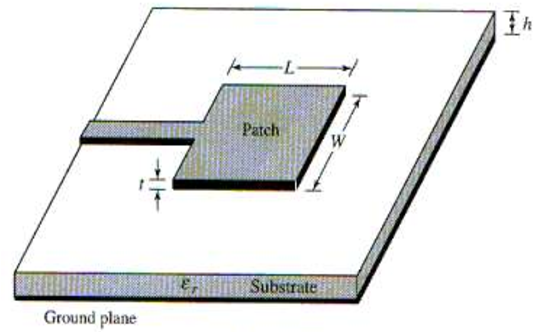
\includegraphics[width=0.5\textwidth]{patch-antenna-structure.png}
    %\end{subfigure}
    \caption{The basic structure of a patch antenna. This particular antenna is being fed with a microstrip. The ground, and the patch are conductors. The substrate is a dielectric. \cite{girase2014design}}
\end{figure}

However, these very rudimentary patch antennas were too large to be effectively used in hand held devices. Like all antennas, patch antennas (PAs) radiate most efficiently when their length is one-half of the wavelength they emit \cite{khan2015microstrip}. For instance, if one wanted to design a PA which radiated at a frequency of $900$ MHz, then, without using any of the miniaturization techniques discussed in this paper, they would need their PA to have a length of around $33$ cm, which is too big to be used in many applications. Besides its large size at lower frequencies, a PA with Figure 1's design would have a narrow frequency band, low efficiency, low power, high Q, poor polarization purity, and spurious feed radiation\cite{balanis2016antenna}. Fortunately, significant effort has gone into addressing these limitations, and a variety of design techniques to mitigate these limitations have been created\cite{balanis2016antenna}. Furthermore, PAs have also been investigated theoretically, and theories to describe the operating mechanism of most PAs have been created. However, the theories describing PA operation are mathematically dense, and are quite challenging to read. This unapproachability in theory leads to obfuscation on both the theory of PA operation, and research associated with it. One of the most intuitive high level ways of describing antennas is visually. While antenna simulation software does exist, it seems like nobody has used it provide a surface level introduction to patch antennas. This paper intends to do so, using the antenna simulation software known as HFSS, by Ansys. HFSS is a 3D electro-magnetic field simulator, used by RF engineers to design antennas, but it can also be used to visualize the fields in patch antennas, thereby giving an intuitive explanation of why certain antenna designs work, and others don't.

This paper will first provide a theoretical overview of how antennas in general emit radiation, as well as explain the properties of AC current that allow for radiation to be created. Next this paper will use HFSS to provide a visual explanation of the radiation mechanism of a basic PA, as well as show some of its properties. None of the information presented here is particularly novel, however, the mechanism behind PA operation is fascinating in its own right. This paper seeks to review PA operation qualitatively.              
\section{Electromagnetic Radiation}  

Before discussing patch antennas, it is important to understand how electromagnetic radiation is created in the first place. Unlike light bulbs, which generate light via the energy released by electrons decaying to lower energy levels inside atoms, antennas radiate via a completely different principle.

First, consider the electric field around some point charge, in some inertial reference frame. The electric field lines will be uniformly distributed, pointing either towards, or away from the source, depending on the charge of the source\cite{schroeder}. Next, consider a case where the charge is moving at some velocity $v_1$, and is then instantaneously accelerated to a higher velocity $v_2$. At this point, the frame of the charge has changed, and the E-field also changes.   

\begin{figure}[h]
    \begin{subfigure}{0.5\textwidth}
    \centering
    	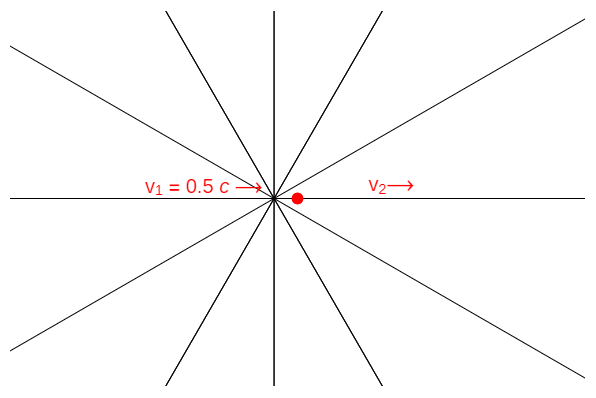
\includegraphics[width=0.9\textwidth]{charge-moving-at-v1.png}
    \end{subfigure}
    \begin{subfigure}{0.5\textwidth}
    	\centering
    	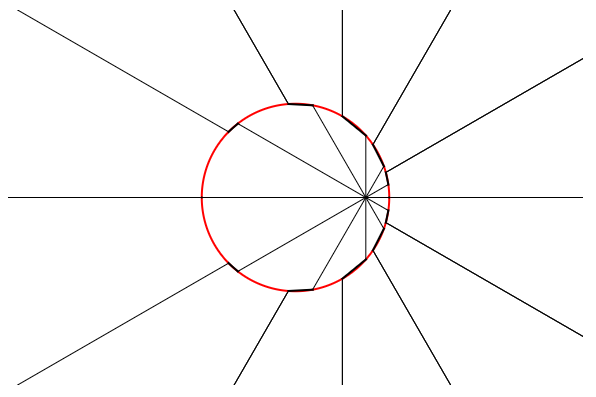
\includegraphics[width=0.9\textwidth]{charge-moving-at-v2.png}
    \end{subfigure}
    \caption{\cite{wolframwave} The electric field around a point charge at two steps in time. On the left is the electric field around a point charge moving at velocity $v_1$. On the right is the electric field around a point charge which has just instantaneous accelerated to a greater velocity $v_2$. When the charge accelerates, the new electric field lines are no longer align with the old electric field lines. }
\end{figure} 

Since the transfer of information is capped by the speed of light, the change to the E-field must also propagate at the speed of light, resulting in a region which was in the old reference frame, and a region which is in the new reference frame. But since the transfer of information is capped by the speed of light, the change to the E-field must also propagate at the speed of light, resulting in a region which was in the old reference frame, and a region which is in the new reference frame. The E-field lines do not align in these two regions. However, broken, or discontinuous electric field lines are not allowed, as that would violate Gauss's law. As a result, the electric field lines must connect from the frame where the velocity of the charge was $v_1$ to the frame with velocity $v_2$ \cite{schroeder}. There is therefore a bend, or kink in the electric field, which propagates to infinity at the speed of light \cite{schroeder}. In this example, the charge accelerated instantaneously from one velocity to the next. This obviously does not happen in reality, but the principle for the bending of the electric field still holds.

Now consider the electric field created by two opposite charges. The E-field points from the positive to the negative charge as shown in figure 3. 

\begin{figure}[h]
    %\begin{subfigure}{0.5\textwidth}
    \centering
    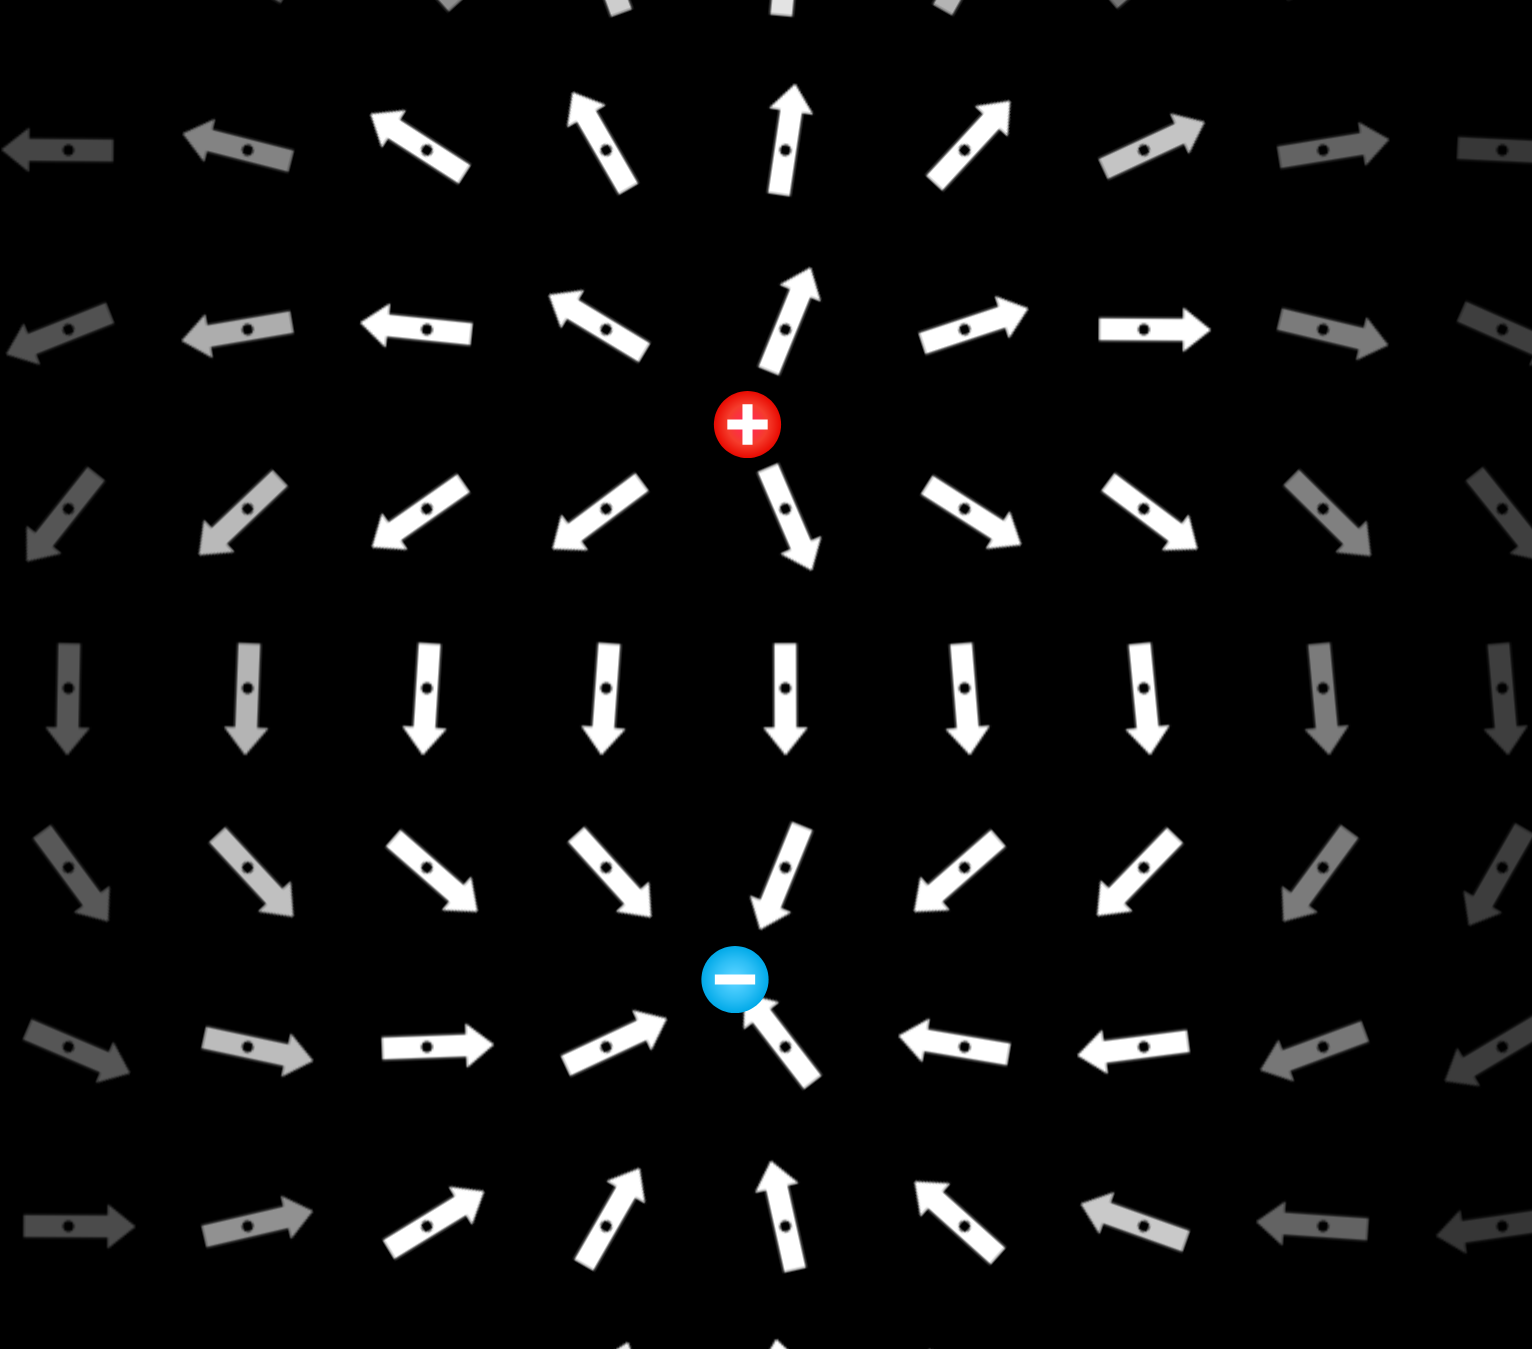
\includegraphics[width=0.3\textwidth]{positive-negative-EField.png}
    %\end{subfigure}
    \caption{The electric field around two point charges of equal magnitude, but of opposite sign.}
\end{figure} 

For the sake of simplicity, only consider one electric field line. Next, suppose that the two charges are oscillating towards each other, as shown in figure 4. The charges are moving sinusoidally (simple harmonic motion), so they are constantly experiencing an acceleration. Initially, the E-field points from the positive charge to the negative charge. As the two charges accelerate towards each other, the E-field starts to kink due to the changing reference frame of the two charges. When the two charges are very close to each other, the E-field is negligible, since the signs of the charges cancel. However, the previous E-field is still propagating outwards, and so the ends of the field lines, which started and ended on the charges, join together to create a closed loop. This loop is the radiation emitted.

\begin{figure}[h]
    \centering
    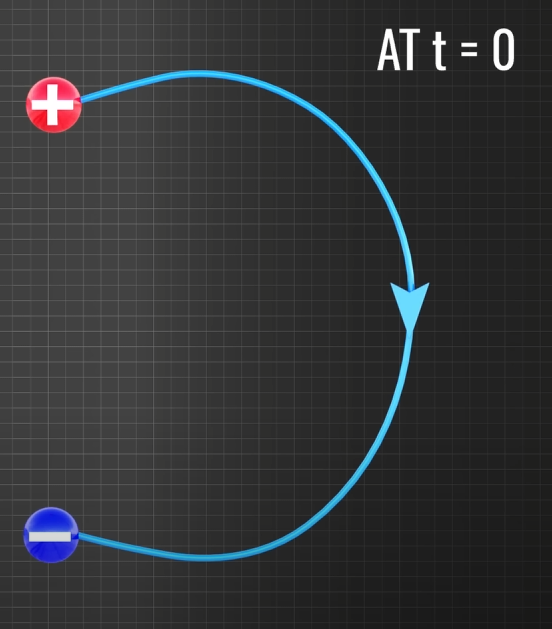
\includegraphics[width=0.20\textwidth]{dipole-at-t0.png} 
    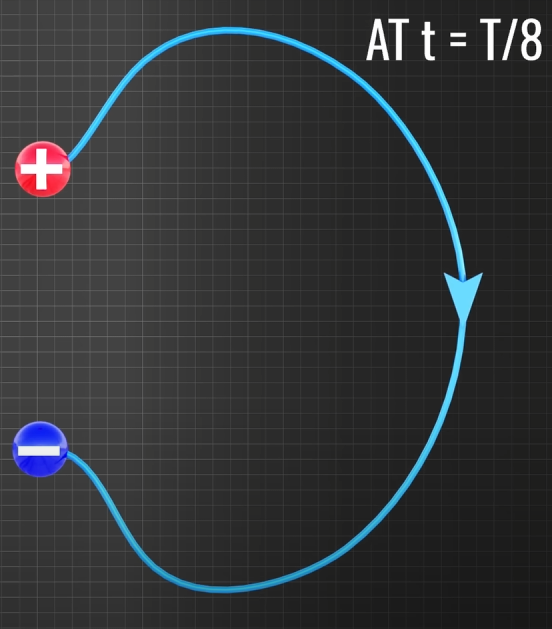
\includegraphics[width=0.20\textwidth]{dipole-at-t1.png}
    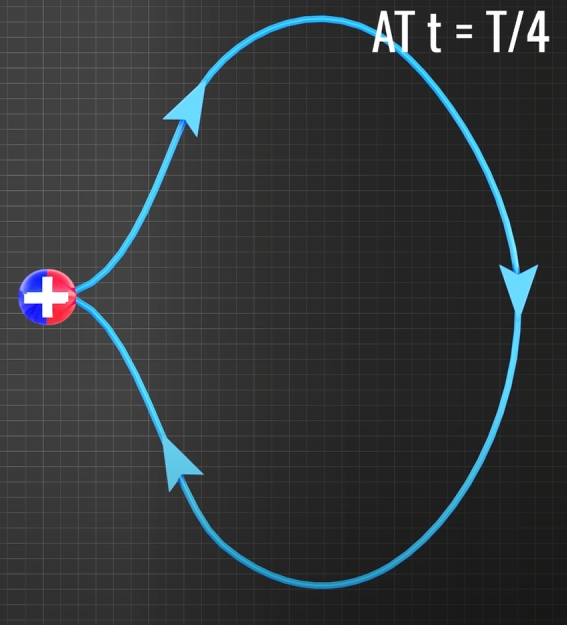
\includegraphics[width=0.20\textwidth]{dipole-at-t2.png}
    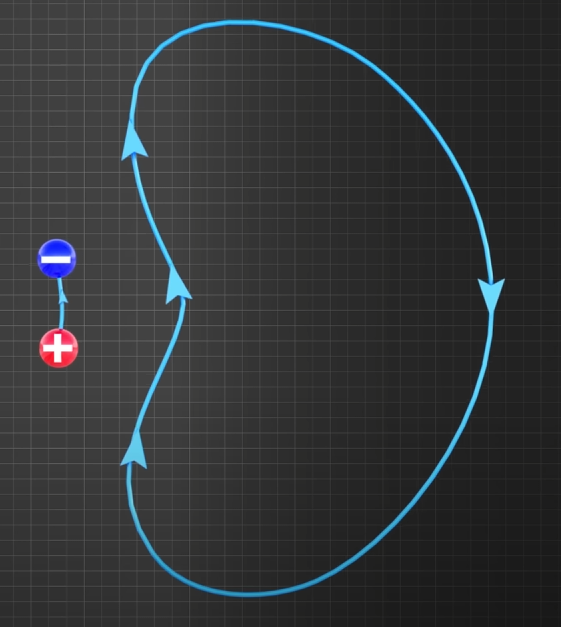
\includegraphics[width=0.20\textwidth]{dipole-at-t3.png}
    \caption{The creation of an electromagnetic wave via the oscillation of a positive and negative charge. Note that this is just the electric portion of the wave. The magnetic portion of the wave is not shown here.}
\end{figure}

It is important to remember that there is also a magnetic field, which is perpendicular to the electric field. It also may be tempting consider the closed E-field loop as one complete wave. However, observe that the charges have not fully returned to their starting positions, and therefore have not yet completed a full oscillation. For this reason, the one closed field loop shown in figure 4 is actually half of the emitted signal, and the other half will be generated when the charges oscillate back to their original positions. It follows that the wavelength of the radiation emitted is equal to the length between two electric field wave fronts, oriented in the same direction. As such, the rightmost image in figure 4 has one half the wavelength of the radiation emitted by the charges.

\section{Properties of Alternating Current}

Although the previous example of two oscillating charges was useful to create a conceptual idea of how EM radiation is generated, it is obviously not how EM waves are generated in antennas. To create the oscillating charges, patch antennas exploit a unique property of alternating current (AC). Consider what happens when an AC source is connected to an open circuit. When the current reaches the end of the line, instead of merely dissipating, the current is reflected in the opposite direction which it came. This leads to a standing wave forming on the wire, due to the interference of identical waves traveling in opposite directions. This standing wave produces an electric field similar to the electric field produced by the oscillating charges in the previous example. 

\section{Patch Antenna Characteristics}

As shown in figure 1, a basic patch antenna consists of a very thin metallic strip (the patch), placed a small fraction of a wavelength above a metallic ground plane. While patches are usually either rectangular or circular\cite{khan2015microstrip}, numerous other shapes have been investigated\cite{balanis2016antenna}. In between the patch, and ground plane, is a dielectric. Dielectrics are electronic insulators which can be polarized by an external electric field. 

\begin{figure}[h]
    %\begin{subfigure}{0.5\textwidth}
    \centering
    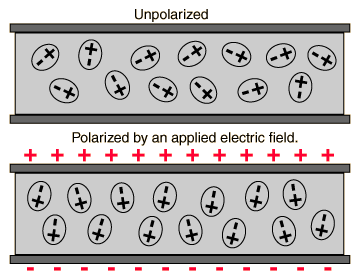
\includegraphics[width=0.3\textwidth]{dielectric.png}
    %\end{subfigure}
    \caption{A dielectric with and without an applied E-field. The dielectric constant $\epsilon_r$ (relative permittivity) is a measure of how much the atoms in the dielectric align to the external E-field. Dielectrics with low $\epsilon_r$ will polarize less to the external E-field, compared to high $\epsilon_r$ dielectrics.}
\end{figure}

Numerous dielectric materials are used in PAs. Most of these materials will have dielectric constants in the range of $2.2$ to $12$\cite{balanis2016antenna}. 
\section{Radiation Mechanisms of Patch Antennas}

The three most popular model used to describe patch antennas are, the transmission line model, the cavity model, and the full wave model\cite{balanis2016antenna}. Since the transmission line model gives the best visual insight\cite{balanis2016antenna} into patch antenna operation, this model will be used. It should be noted however, that the transmission line model is only valid for rectangular patch antennas, and doesn't give the most accurate results\cite{balanis2016antenna}. As a result, the results from both the cavity wave model, and the full wave model will be included. More information on the cavity model can be found here \cite{balanis2016antenna}. 


\section{E-Field on the Patch}
 

\begin{figure}[h]
    %\begin{subfigure}{0.5\textwidth}
    \centering
    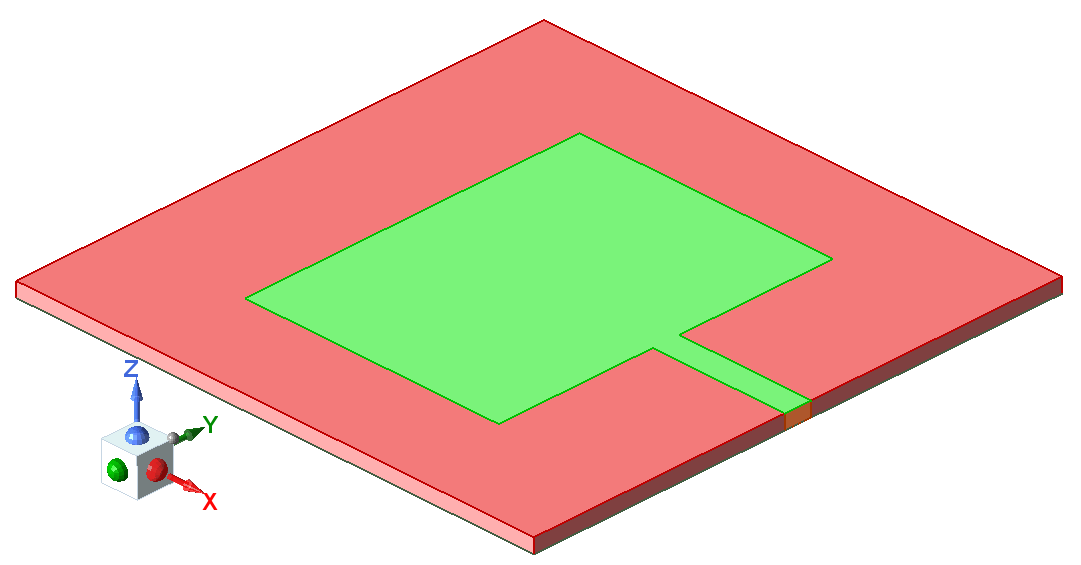
\includegraphics[width=0.5\textwidth]{2.4GHz-basic-pa.png}
    %\end{subfigure}
    \caption{A basic PA designed in HFSS. This particular PA has been designed to radiate at 2.4 GHz. The green material on top is the patch, with the red material being the substrate. The substrate has a relative permittivity (dielectric constant) of 4.4. There is a ground plane beneath the substrate, although it is not visible here. The entire antenna has dimensions $60 \text{ mm} \times 60 \text{ mm} \times 1.6 \text{ mm}$, in the x,y,z planes, respectively. The patch itself is 29.4 mm long in the x direction, and 38 mm long in the y direction. The thickness of the patch and ground plane is negligible with respect to the substrate thickness. }
\end{figure}

Figure 3 depicts a basic microstrip patch antenna (MPA) that is designed to radiate at 2.4 GHz. When an RF signal is applied to this antenna, at a 2.4 GHz frequency, the patch antenna will radiate EM waves. Although the antenna can radiate at other frequencies, it will radiate less efficiently at those frequencies. The frequency at which an antenna radiates most efficiently is known as the \textit{resonant frequency} of the antenna. A more technical definition of the resonant frequency of an antenna is the frequency at which the impedence of an antenna is purely resistive, the frequency at which the capacitive and inductive reactances cancel each other out. 

The exact radiation mechanism for a rectangular patch antenna can be modeled by treating the patch as an open ended transmission line. When a signal passes through the micro-strip and into the patch itself, the signal travels down the length of the patch, and is reflected upon reaching the far end of the patch. The reflected signal then interferes with the incoming RF signal, to create a standing wave on the patch. This standing wave then allows for the radiation of free space waves. The reflected signal does not travel back into the micro-strip and into the feedline due to the impedence mismatch between the microstrip line and the patch. So, when the reflected signal reaches the other side of the patch, it gets reflected again, and will be reflected until it runs out of energy.   

\begin{figure}[h]
    %\begin{subfigure}{0.5\textwidth}
    \centering
    \includegraphics[width=0.5\textwidth]{basic-patch-antenna-MagE-on-patch.png}
    %\end{subfigure}
    \caption{This depicts the same PA from figure 3, with an RF current applied to the patch. The magnitude of the E-field is being shown on the patch, with the RF current applied. A stronger E-field at some point is represented by a warmer color.}
\end{figure}

As observed in figure 4, the E-field is strongest around the edges of the patch, and decreases rapidly towards the center of the patch. This is due to the skin effect, where at either high frequencies, or high currents, the current through a conductor gets pushed out to the outermost edges. 

\begin{figure}[h]
    %\begin{subfigure}{0.5\textwidth}
    \centering
    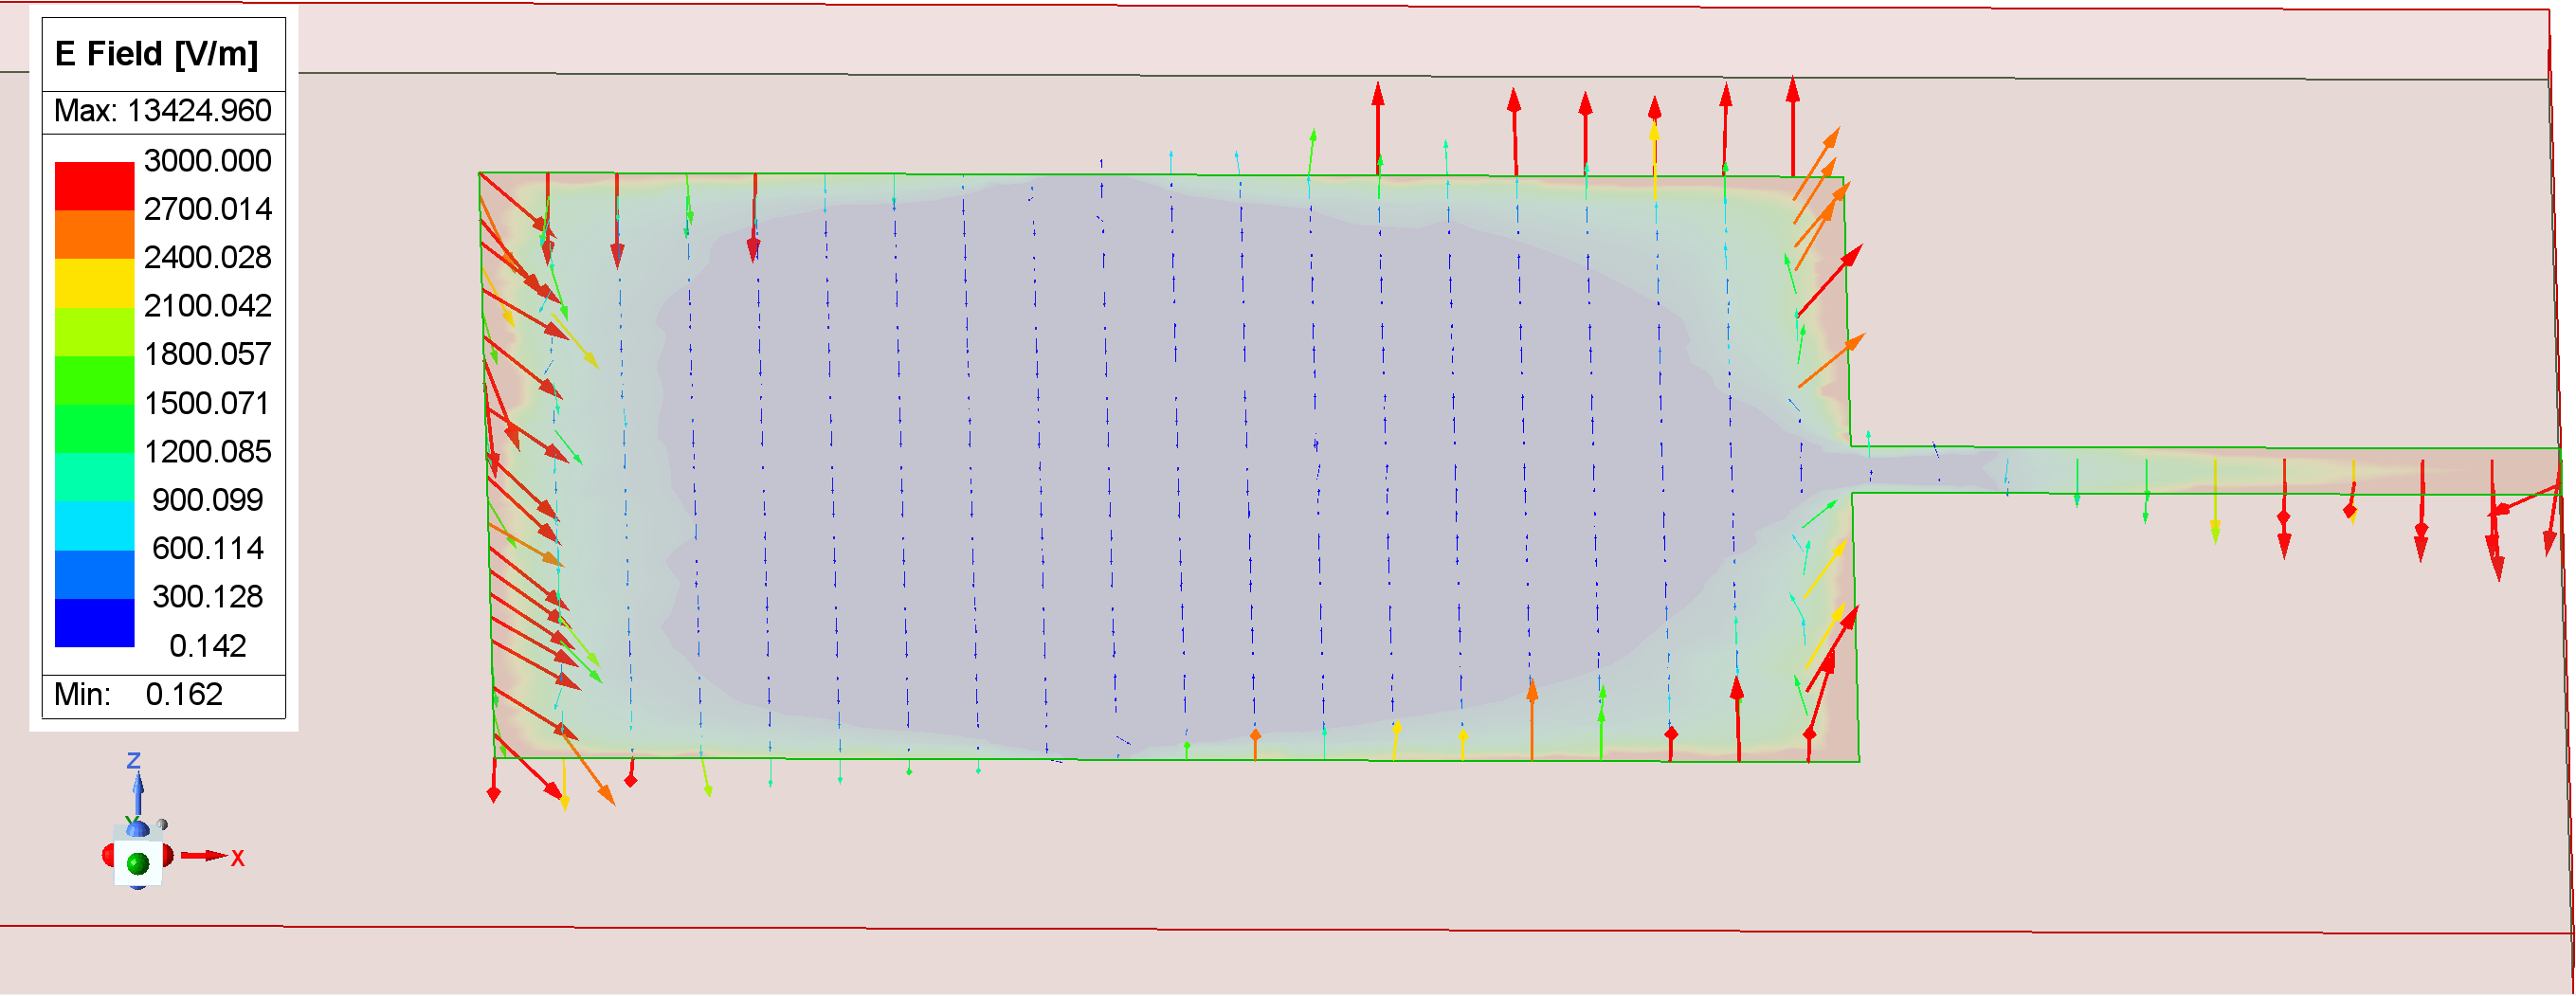
\includegraphics[width=0.5\textwidth]{basic-patch-antenna-VecE-onPatch-t0.png}
    %\end{subfigure}
    \caption{This shows the E-field as a vector on the patch. It is clear that the E-field is strongest on the outside edge of the patch, while the center of the patch has virtually no E-field. Furthermore, the E-field at either end of the patch is not oriented solely in the z direction, which is due to the curvature of the edge of the patch.}
\end{figure}
  

\section{Near Field Radiation}

To better understand the far field radiation pattern of the patch, first consider the E-field pattern around the patch. As demonstrated in figure 5, the edges of the patch contain the strongest E-field. Consider what would happen if the sources of these strong E-fields was fixed. As time passes, the new surrounding space would conform to these E-fields. An important realization is that the two locations where the E-fields are strongest can be modeled as a pair of opposite electric charges. At a certain distance the E-field will point from one point of strong E-field, to the other point of strong E-field, as shown in figure 6.

\begin{figure}[h]
    %\begin{subfigure}{0.5\textwidth}
    \centering
    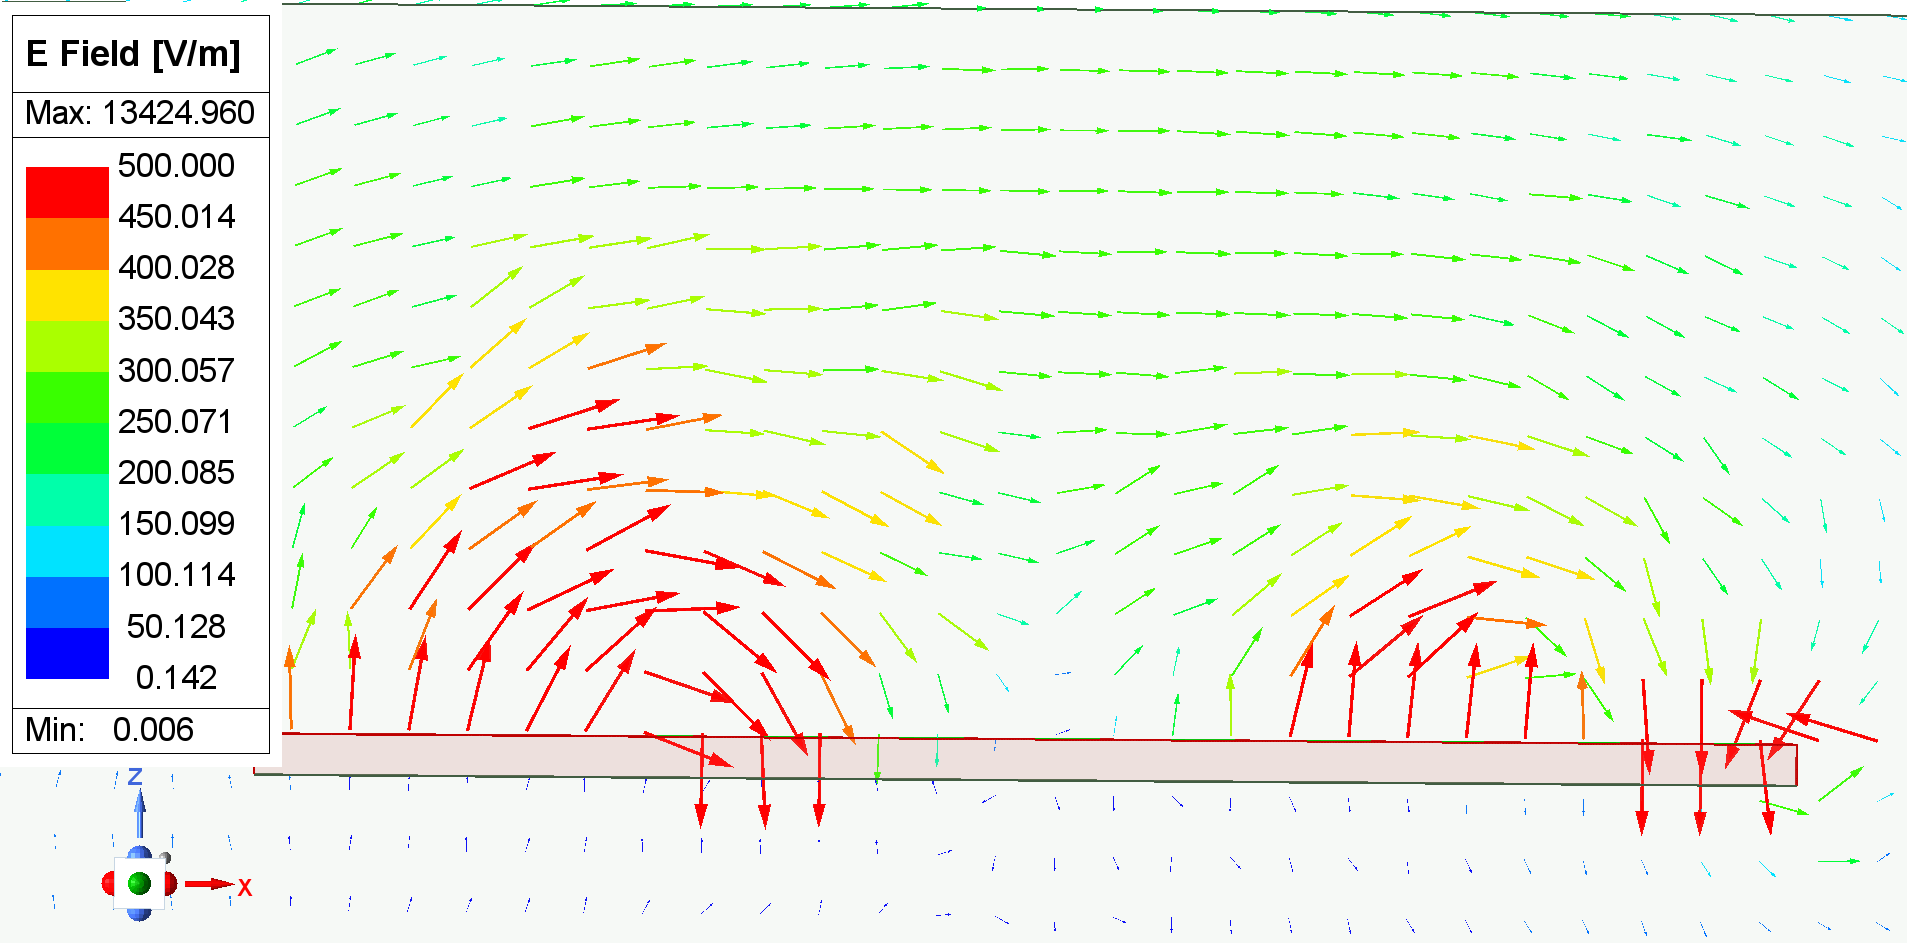
\includegraphics[width=0.5\textwidth]{basic-patch-antenna-near-Efield.png}
    %\end{subfigure}
    \caption{This shows the E-field near the patch, at a snapshot in time. Observe that at a certain distance the E-field appears to travel from one point of high E-field strength to the other. In other words, from a certain distance the overall pattern of the E-field matches the expected pattern of an E-field formed by a positive and negative pair of charges.}
\end{figure}  
This connected E-field will extend out towards infinity (assuming that the charges remain fixed), and is crucial to understanding the far field radiation of the antenna. 

\section{Far Field Radiation}

As the standing wave on the patch oscillates back and forth, the resulting oscillations cause ripples in the field near the patch. As the E-field propagates outwards, the standing wave on the patch flips back and forth, mimicking the oscillating electric charges used to describe EM radiation. At the moment when the standing wave is null, the E-field closes, just like in the charged particles example, and the radiation radiates away from the antenna. The oscillation continues, and radiation is generated. Figure 10 demonstrates the formation of a free traveling EM wave, created by the patch antenna.

\begin{figure}[h]
    \centering
    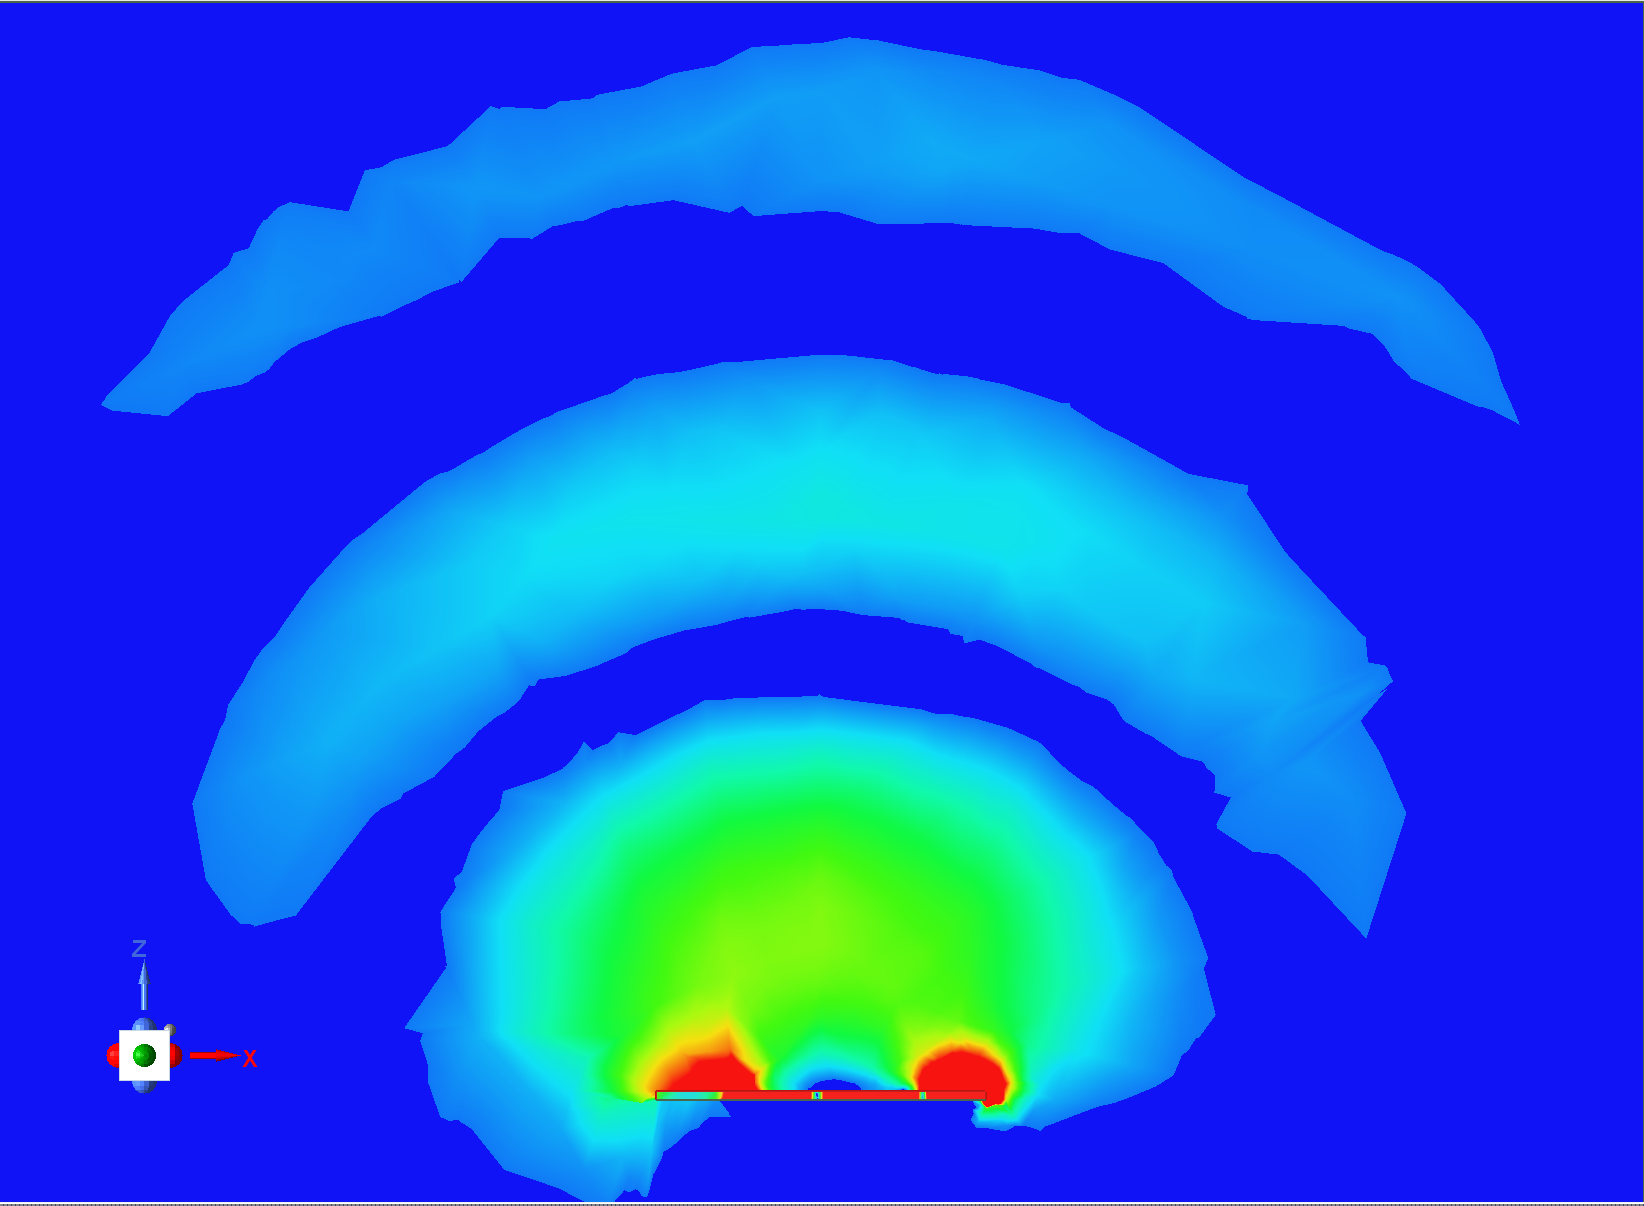
\includegraphics[width=0.35\textwidth]{basic-patch-antenna-radiating-t0.png} 
    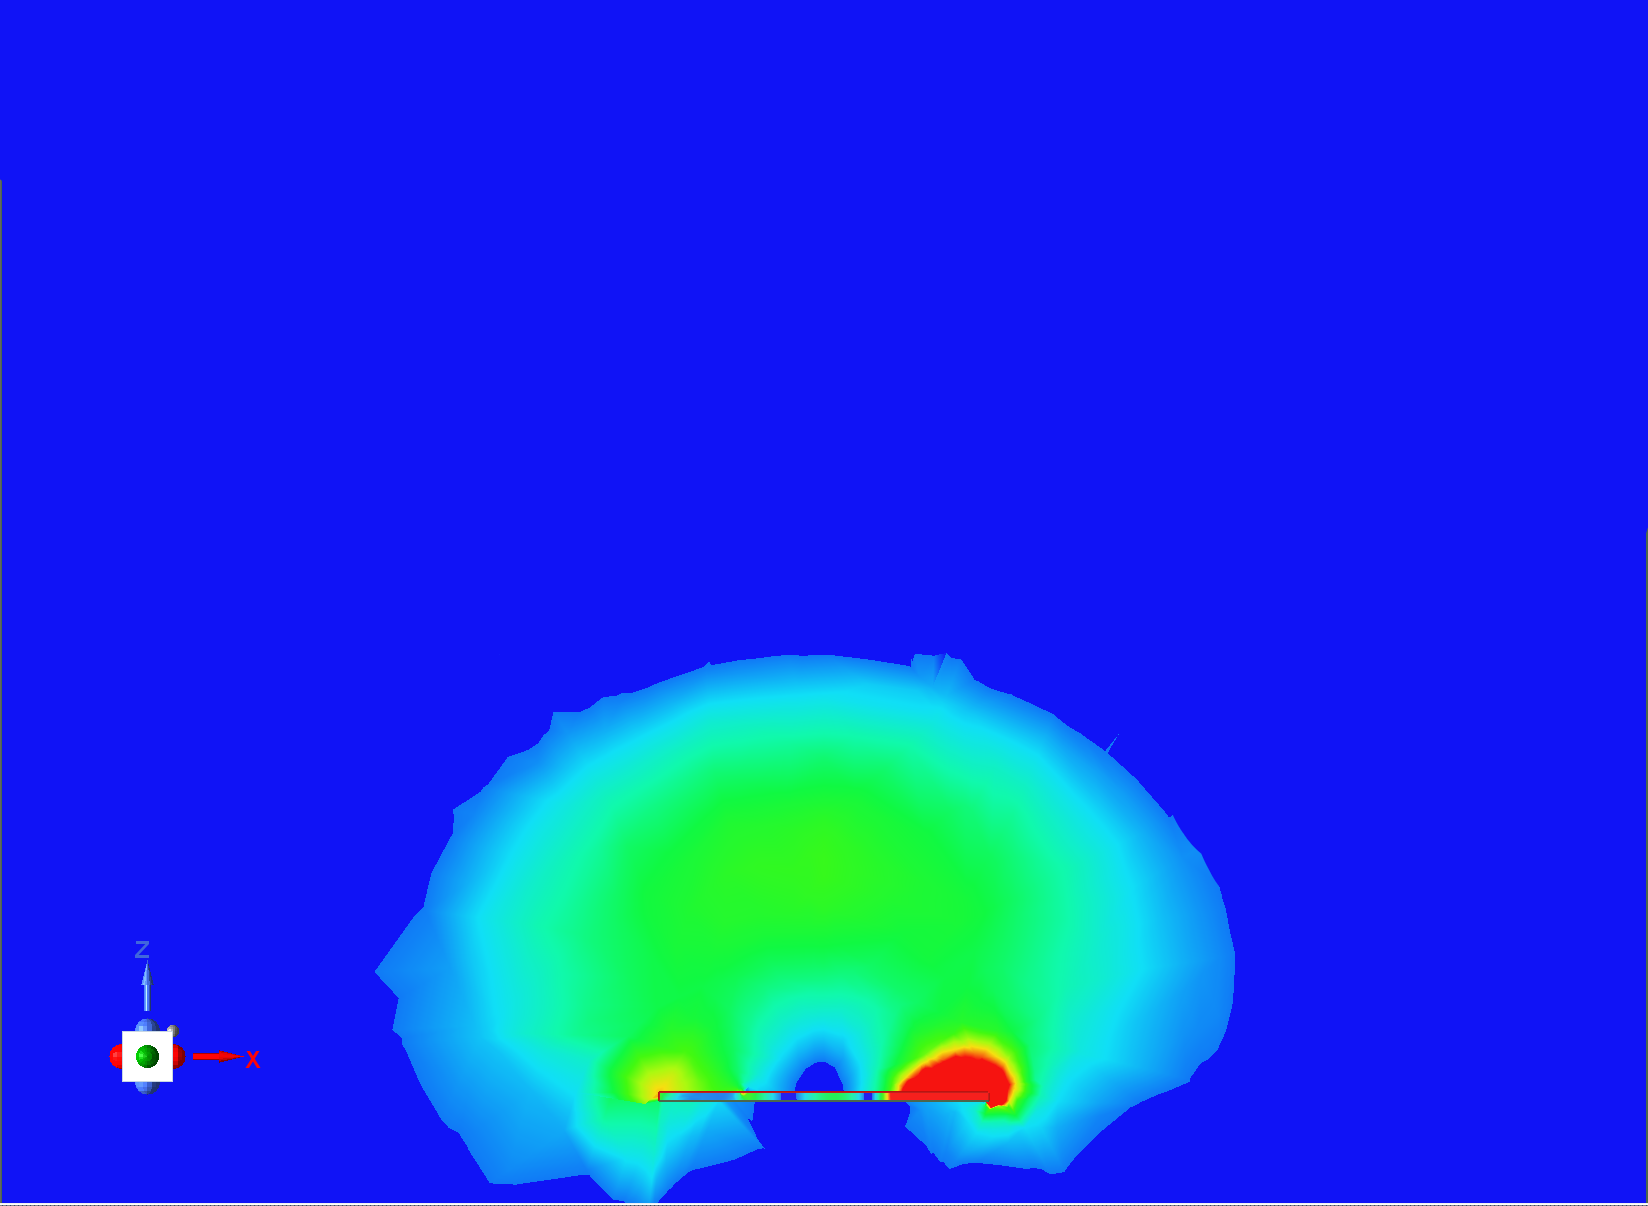
\includegraphics[width=0.35\textwidth]{basic-patch-antenna-radiating-t1.png}
    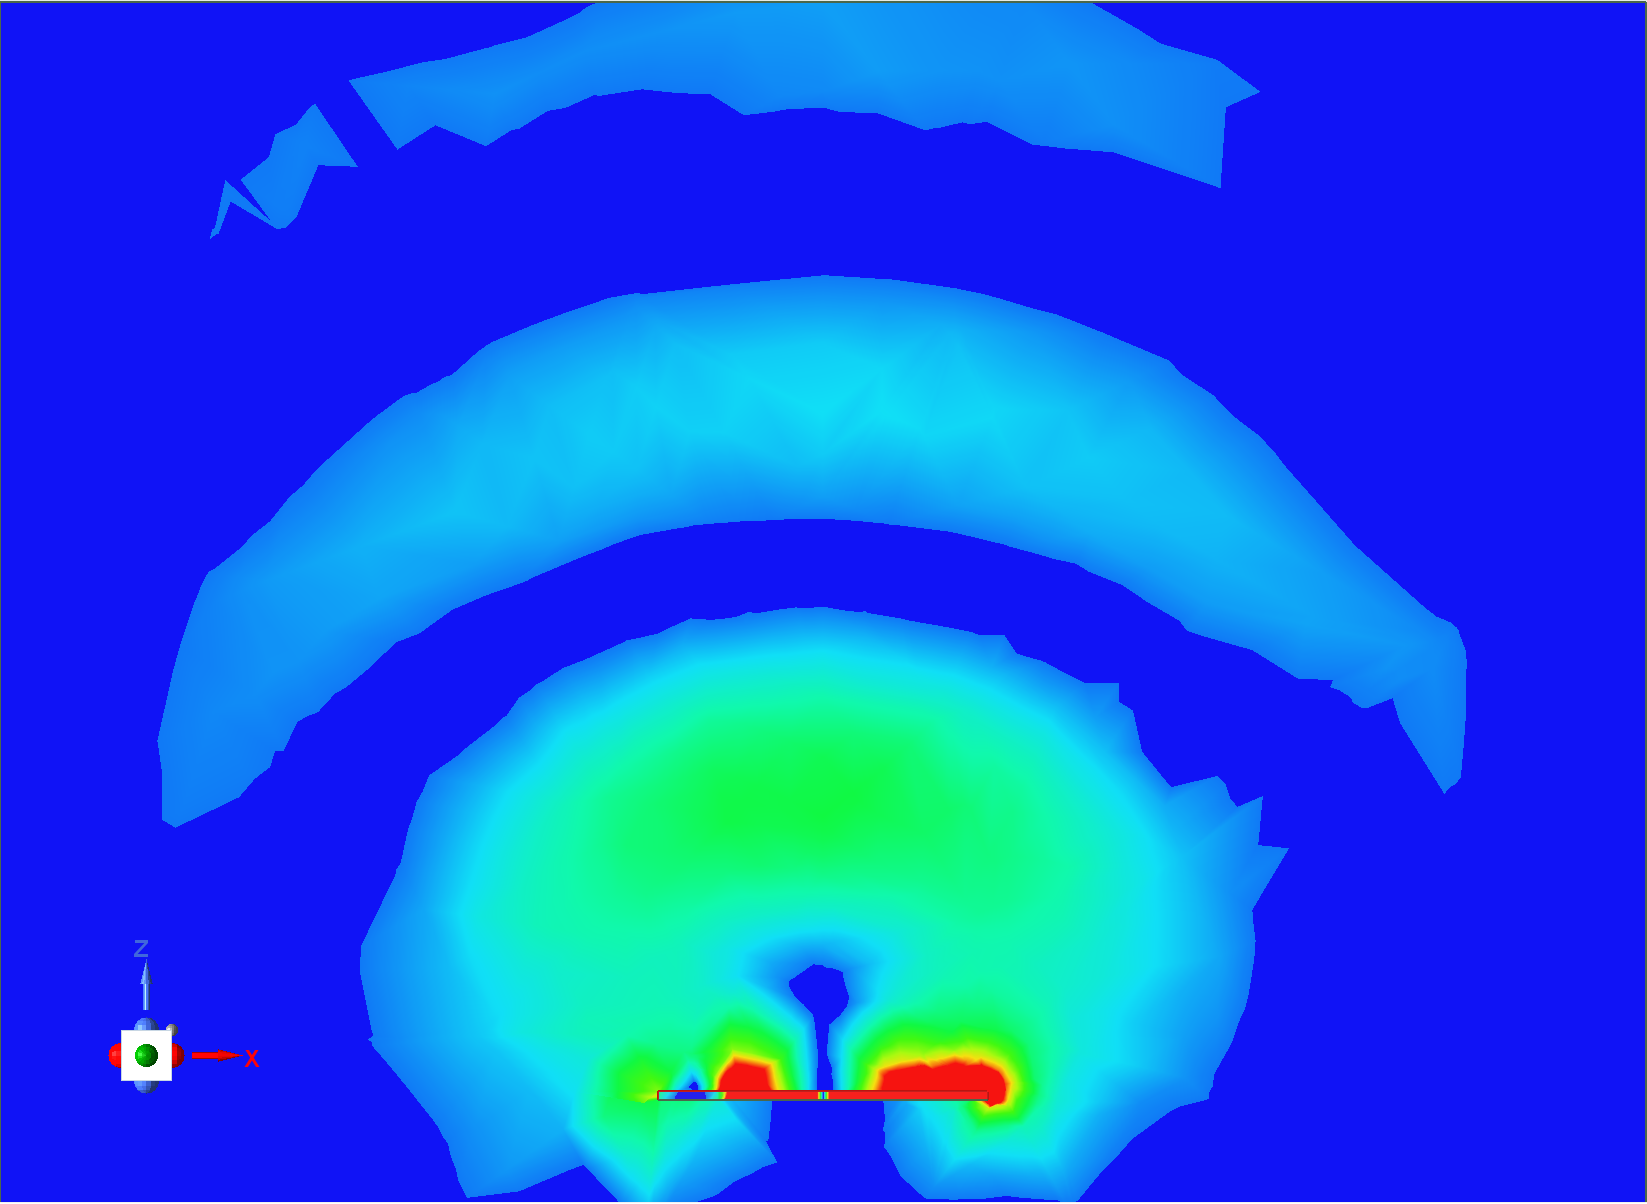
\includegraphics[width=0.35\textwidth]{basic-patch-antenna-radiating-t2.png}
    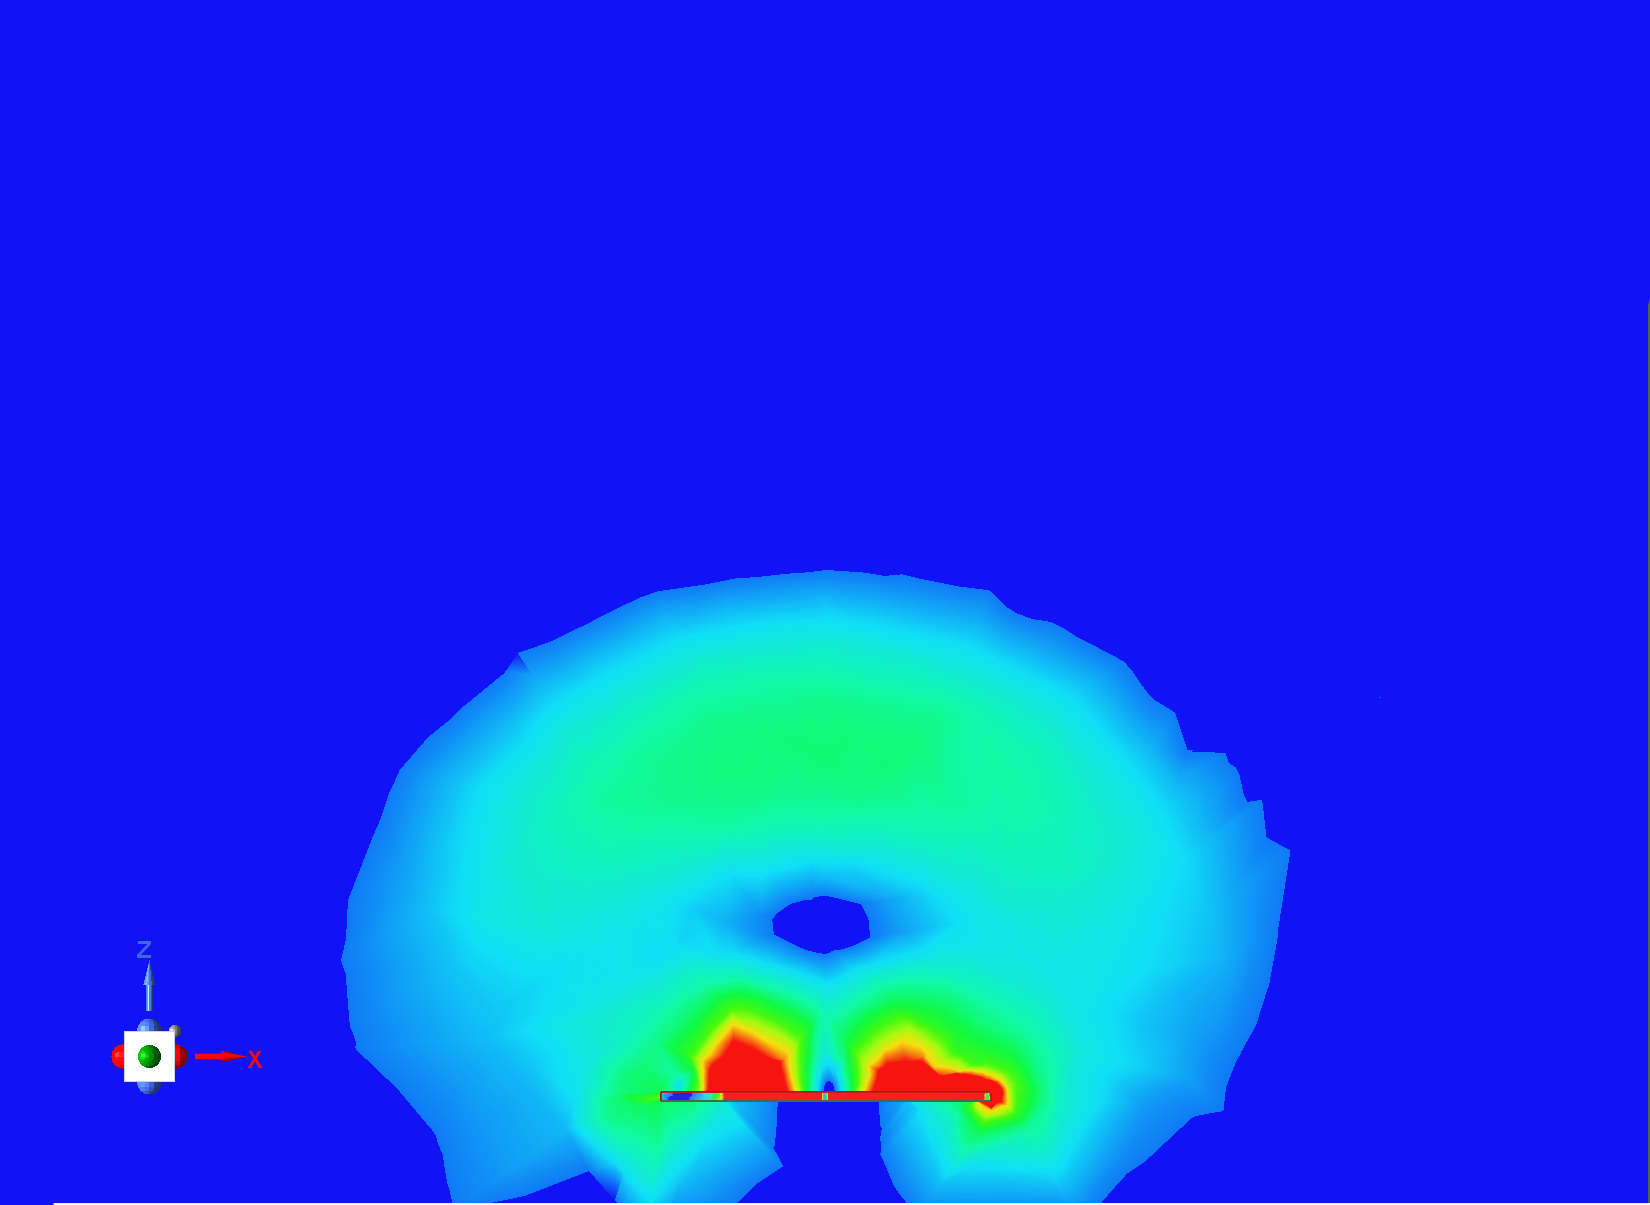
\includegraphics[width=0.35\textwidth]{basic-patch-antenna-radiating-t3.png}
    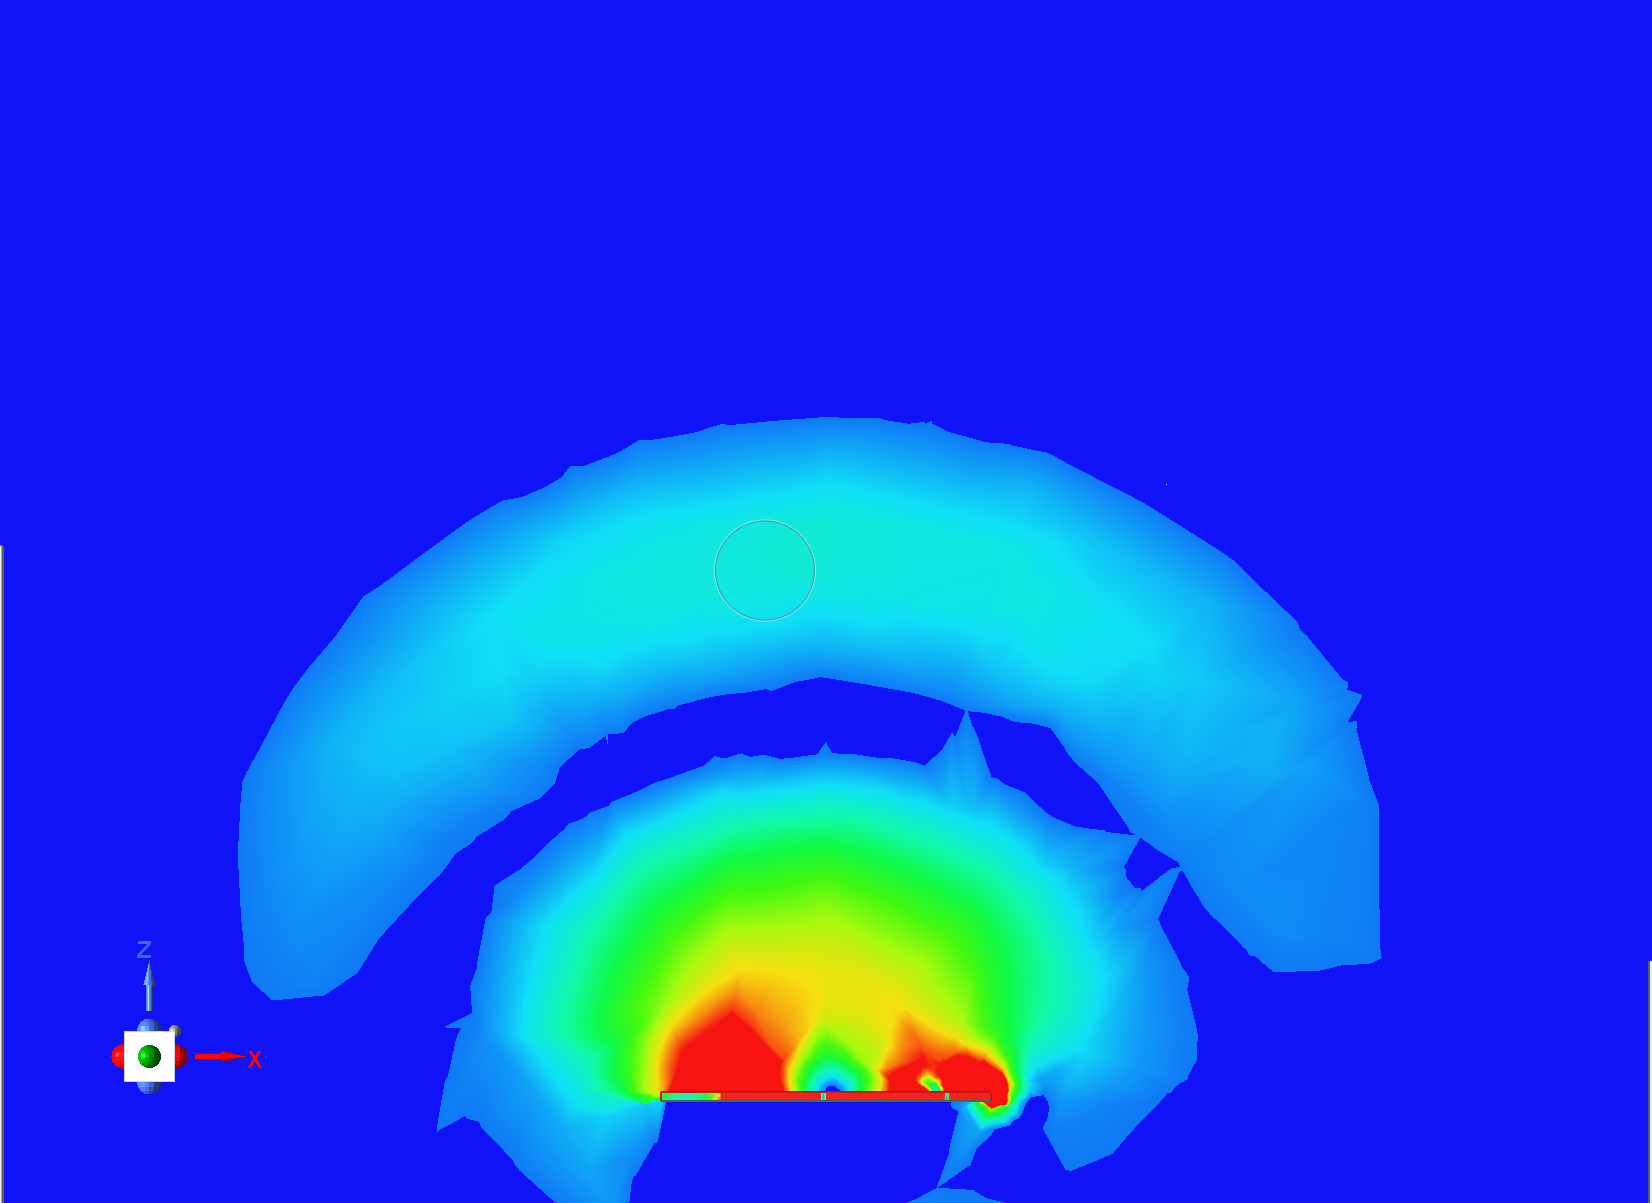
\includegraphics[width=0.35\textwidth]{basic-patch-antenna-radiating-t4.png}
    \caption{The creation of an electromagnetic wave from a patch antenna, at different points in time. The time of each image is from left to right, top to bottom. The bottom image shows a wave detached from the antenna.}
\end{figure} 

\section{Properties}

The simulation shows that patch antennas are broadside radiators, in that they radiate almost all of their energy parallel to the normal of the patch. This leads to patch antennas having a high directivitty. They are generally considered to have moderate gain amongst antennas\cite{khan2015microstrip}. The two combined properties make patch antennas useful for situations where the positions of the receiver and transmitter are known, so that the antenna may efficiently transmit power to the destination. 
\newpage
\begin{figure}[h]
    %\begin{subfigure}{0.5\textwidth}
    \centering
    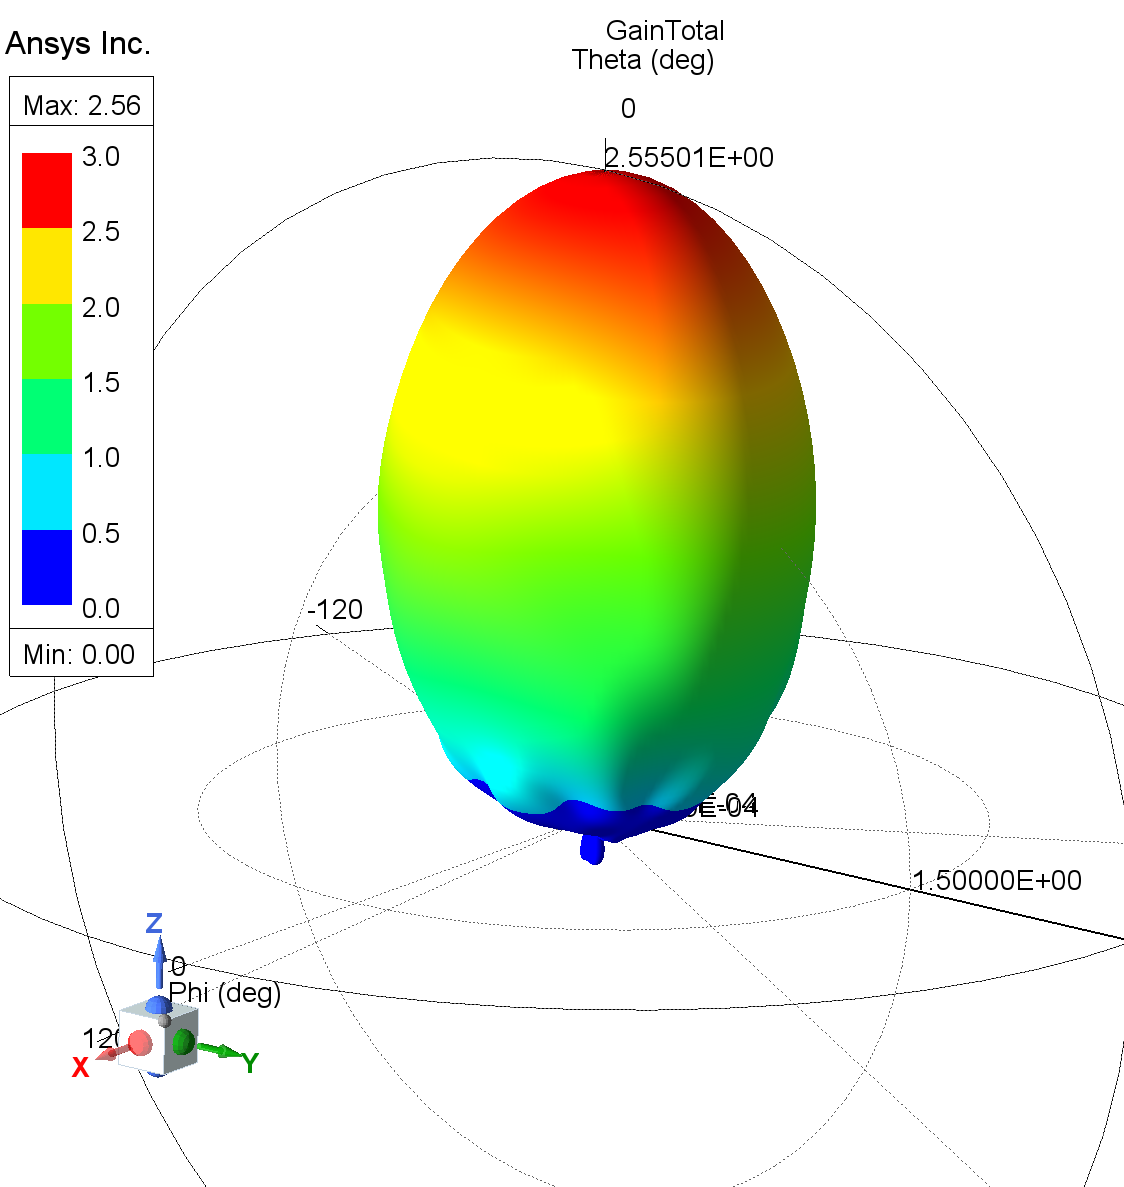
\includegraphics[width=0.45\textwidth]{basic-patch-antenna-gain.png}
    %\end{subfigure}
    \caption{This shows a 3 dimensional polar plot of the gain of the patch antenna described in earlier sections.}
\end{figure}

Besides their high directivitty, the patch antenna presented here has a very narrow bandwidth. Bandwidth refers to the number of frequencies on which the antenna can efficiently radiate power. This is typical for basic patch antennas\cite{balanis2016antenna}. Although having a larger bandwidth is generally preferable in antenna design, some applications, such as military communication, desire antennas with narrow bandwidth\cite{balanis2016antenna}, so the narrow bandwidth is not necessarily undesirable.

\begin{figure}[h]
    %\begin{subfigure}{0.5\textwidth}
    \centering
    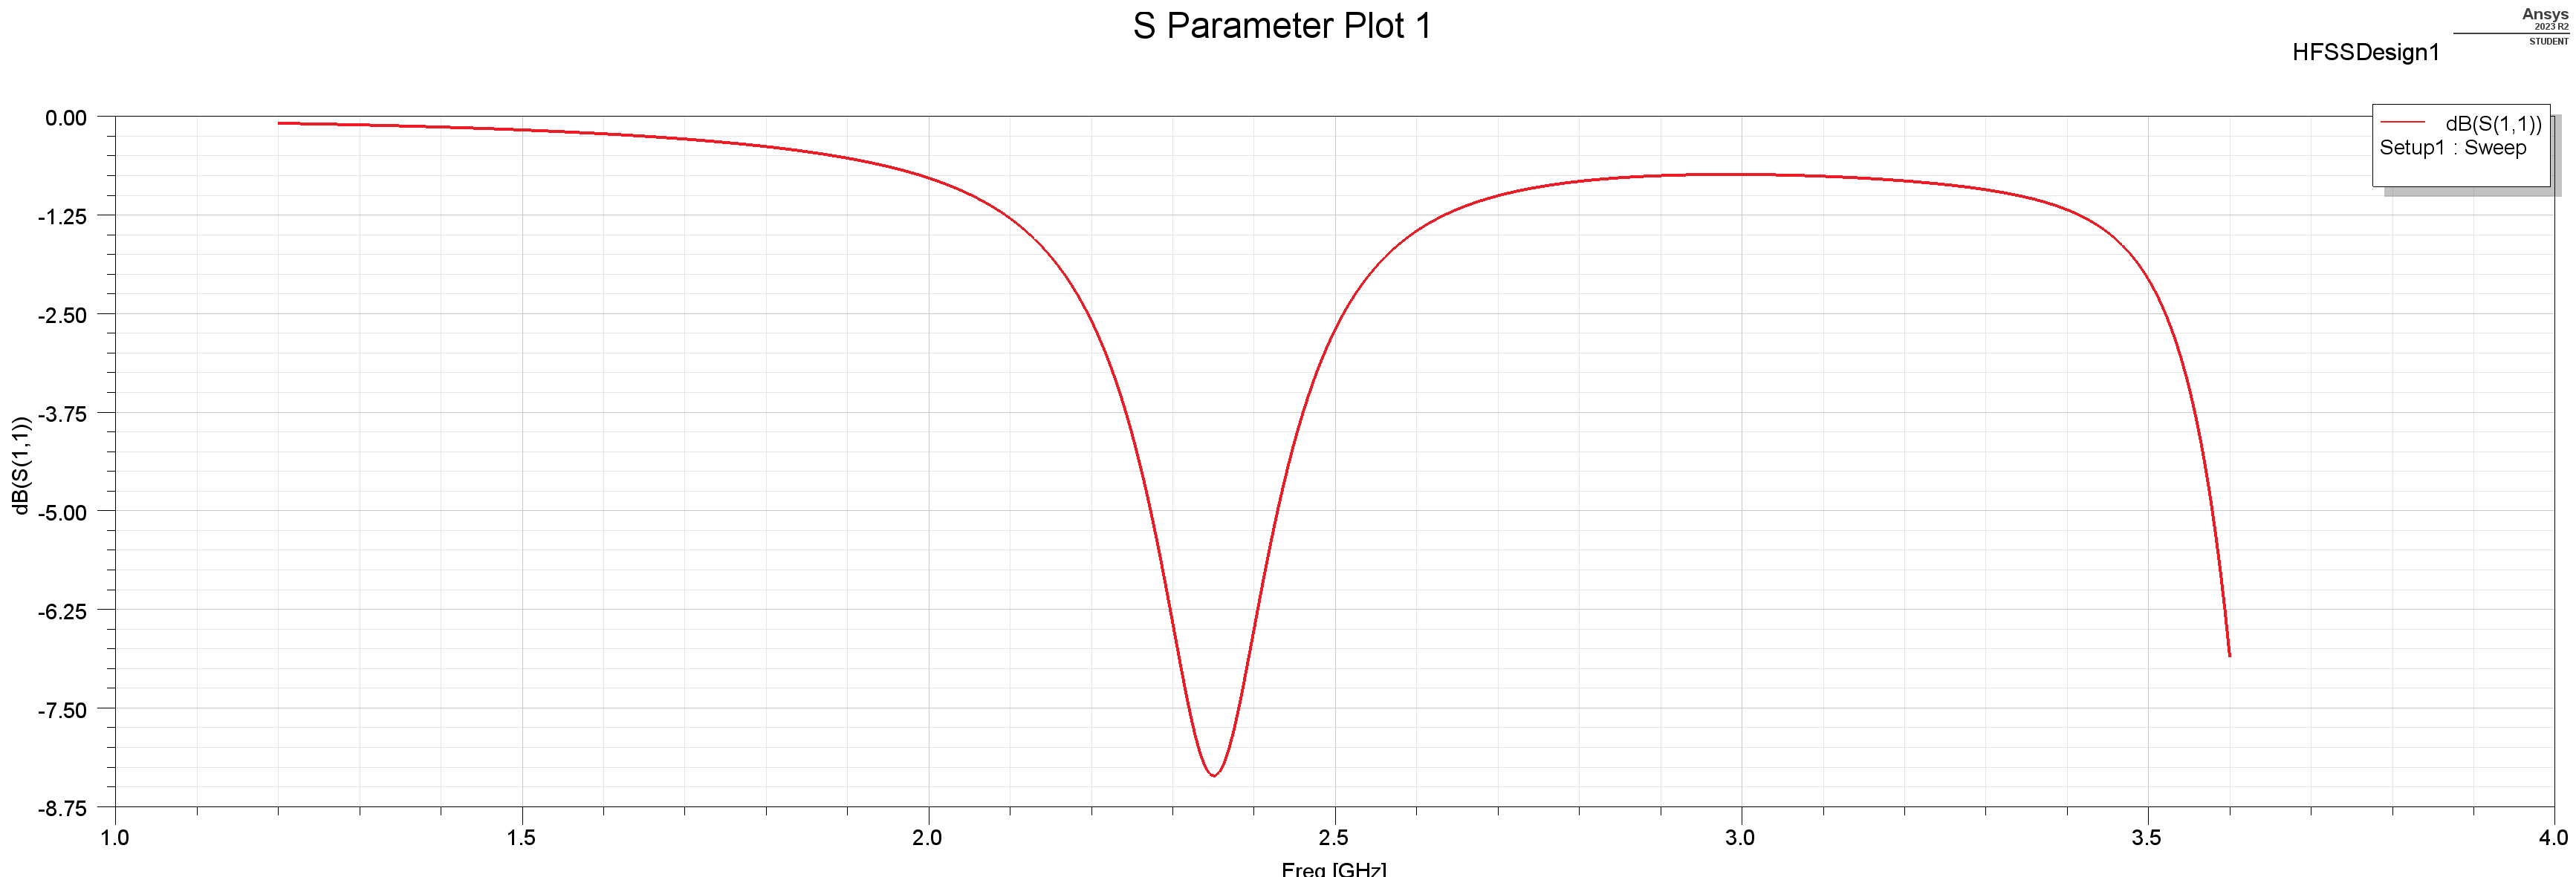
\includegraphics[width=0.9\textwidth]{basic-patch-antenna-splot.png}
    %\end{subfigure}
    \caption{The graph shows the frequency of the signal supplied to the antenna vs the reflection coefficient in decibels. The reflection coefficient of an antenna describes how much of the power being input into an antenna is reflected back to form a standing wave, and thus radiate. A negative reflection coefficient as seen here means that the reflected wave is inverted.}
\end{figure}

From figure 12, its clear that the antenna radiates most efficiently at around 2.35 GHz. The narrow bandwidth of the antenna is obvious, due to the narrow valley centered at 2.35 GHz. There is also a drop off towards the far right side of the plot. This is because standing waves can have different resonant modes. The 2.35 GHz frequency happens to be the lowest mode for this antenna design, however, higher modes do also exist.

\section{Conclusion}

Patch antennas are some of the most ubiquitous antennas today, and the body of knowledge accompanying them is vast. This paper gave a mere glimpse into the operation of patch antennas. Although the explanation given for the radiation mechanism for patch antennas given here does adequately explain the operation of a basic rectangular patch antenna, it is insufficient to describe patch antenna radiation as a whole\cite{balanis2016antenna}. Patch antennas have been made with an enormous number of various shapes, and the theory used here would not be able to adequately describe their operation. To address this shortcoming, researchers have worked on other theories to describe patch antenna operation, and many have been created. In addition, much research has been done to overcome the shortcomings of patch antennas, and numerous innovations have been made\cite{balanis2016antenna}. Today, patch antennas can be miniaturized, can be circularly polarized, can have their bandwidth widened, can be used in arrays, and much more. 

\newpage
\bibliographystyle{IEEEtran}
\bibliography{main}
%\printbibliography


\end{document}
